\resizebox{0.2\textwidth}{!}{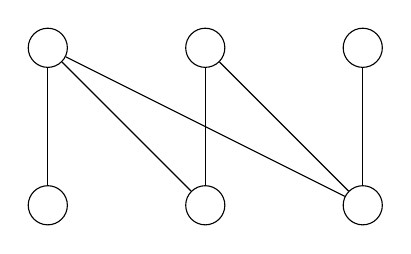
\begin{tikzpicture} [myv/.style={circle, draw, inner sep=5pt},myv1/.style={circle, draw, inner sep=0pt,color=white},myv2/.style={rectangle, draw, dotted,  inner sep=2pt,line width = 0.5mm}]
 % \node [label=above: $\Large{r}$](z)  at (0,4) {};

  \node[myv] (a) at (0,0) {};
  \node[myv] (b) at (0,2) {};
  \node[myv] (c) at (2,0) {};

  \node[circle, draw, inner sep=5pt] (d) at (2,2) {};
  \node[myv] (e) at (4,0) {};
  \node[circle, draw, inner sep=5pt] (f) at (4,2) {};
  
    \draw (a) -- (b);
    \draw (b) -- (c);
    \draw (c) -- (d);
    \draw (d) -- (e);
    \draw (e) -- (f);
    \draw (e) -- (b);
    
    
   
  

\end{tikzpicture}}
